%!TEX root = ./main.tex
\section{Linear Maps}
\begin{center}
    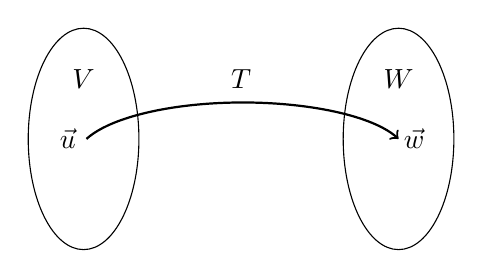
\begin{tikzpicture}
        \draw (2,0) ellipse (20pt and 40pt);
        \draw[] (-2,0) ellipse (20pt and 40pt);
        \draw[<-, thick] (2,0) arc (20:160: 60pt and 20pt);
        \draw (0,1)  node[anchor = north] {$T$};
        \draw (2,1)  node[anchor = north] {$W$}; 
        \draw (-2,1) node[anchor = north] {$V$};
        \draw (-2.2,0) node {$\vec u$};
        \draw (2.2,0) node {$\vec w$};
    \end{tikzpicture}
\end{center}
\subsection{Linear Maps as Vector Space}
Suppose $V$ and $W$ are two linear spaces over $\b F$. $T$ is a function with domain $V$ and codomain $W$. $T$ is called linear iff 
\begin{enumerate}
    \item $T(\vec u_1 + \vec u_2) = T(\vec u_1) + T(\vec u_2)$
    \item $T(\lambda \vec u) = \lambda \cdot T(\vec u)$
\end{enumerate}
$\forall \vec{v}_1, \vec{v}_2 \in V$ and $\forall \vec v_1 \vec v_2 \in V, \forall \lambda\in \b F$.
\begin{example}
    Let $V = \b R^3, W = \b R^4$. Define $T$ as $(x_1, x_2, x_3) \mapsto (x_1,0,0,0)$
\end{example}
\begin{example}
    $T: \c P(x) \to \c P(x)$, where $\displaystyle f(x) \mapsto \int_{10}^x f(x) \ dx$ is a linear map.
\end{example}
\begin{definition}
    $\c L\{V, W\}$ denotes the set of all linear maps from $V$ to $W$. Note that $\c L\{V, W\}$ with $+$ and $\cdot$ becomes a vector space over $\b F$. This requires the additions of functions and multiplications of linear maps by scalars (from $\b F$). Given $T_1, T_2 \in \c L(V,W)$ we define addition as $(T_1 + T_2)(\vec u) := T_1(\vec u) + T_2(\vec u)$, multiplication as $(\lambda T)(\vec u) : = \lambda \cdot T(\vec u)$. 
\end{definition}
\begin{theorem}
    In finite vector space $V,W$, let $\li{\vec u}n$ be a basis for $V$, let $\li{\vec w}m$ be any vectors in $W$. Then there exist a unique linear map $T \in \c L \lb V, W \rb$ such that $T(\vec u_j) = \vec w_j \forall j$.
\end{theorem}
\begin{proof}
    Any vector in $V$ has a unique representation $\alpha_1\vec u_1 + \alpha_2\vec u_2 + \cdots + \alpha_n \vec u_n = \vec u$.  \\ Define $T(u):= \underbrace{\lincomb \alpha {T(\vec u)}n}_{\in W}$ This makes $T$ a linear map from $V$ to $W$. Indeed if $\lambda \in \b F$, then $T(\lambda u) = T(\sum_{j = 1}^n \lambda \alpha_j \vec u_j) = \lambda \sum_{j = 1}^n \alpha_j \vec wj$. Suppose $\tilde T(\vec u_j) = \vec w_j$ for all $j$, then $T = \tilde T$ as a map function by linearity and basis.
\end{proof}
\subsection{Null Space and Range}
\begin{theorem}
    Let $\nul (T):= \lb \vec u \in V : T(\vec u) = 0 \rb$. $\nul (T)$ is a subspace of $V$.
\end{theorem}
\begin{theorem}
    Let $\range (T):= \lb \vec w \in W : T(\vec u) = \vec w \rb$. $\range(T)$ is a subspace of $W$.
\end{theorem}
\begin{proof}
    The proof is trivial and is left as an exercise for the reader.
\end{proof}
\begin{example}
    Let $T: f \to f', V:= \c P(x), W:= \c P(x)$. $\nul(T) = \c P_0(x)$, $\range(T) = \c P_2(x)$. \\
    Let $T: f \to f'', V:= \c P(x), W:= \c P(x)$. $\nul(T) = \c P_1(x)$, $\range(T) = \c P_1(x)$.
\end{example}
\begin{example}
    Find a basis of $\c L (V,W)$ given bases $\lb \li{\vec u}m \rb$ and $\lb \li{\vec w}n \rb$ of $V$ and $W$. \\
    The basis consists of $m \times n$ vectors as follows: 
    \[T_{11} = T(\vec u_1) = \vec w_1, T(\vec u_2) = \vec 0, T(\vec u_3) = \vec 0, \ldots ,T(\vec u_m) = \vec 0\]
    \[T_{12} = T(\vec u_1) = \vec w_2, T(\vec u_2) = \vec 0, T(\vec u_3) = \vec 0, \ldots ,T(\vec u_m) = \vec 0\]
    \[ \cdots \]
    \[T_{mn} = T(\vec u_1) = \vec 0, T(\vec u_2) = \vec 0, T(\vec u_3) = \vec 0, \ldots ,T(\vec u_m) = \vec w_n\]
\end{example}
\begin{example}
    Let $\c U = \lb f : \b R \to \b R : f(x) = f(1-x) \ \forall x \rb$.
    \begin{enumerate}
        \item Show that $\c U$ is a subspace of $f: \b R \to \b R$. 
        
        \item Find a complement.
        \[ \c W  = \lb g : \b R \to \b R : g(x) = -g(1 - x) \ \forall x \rb\]
        
    \end{enumerate}
\end{example}
\begin{proof}
            We can see that the zero function $f(x) = 0$ satisfies the requirement since $0 = 0$ for all  values of $x$. 
            
            Suppose $f(x), g(x) \in \c U$, then we compute \begin{align*}
                (f + g)(x) &= f(x) + g(x) \\
                           &= f(1 - x) + g(1 - x) \\
                           &= (f + g)(1 - x)
            \end{align*}
            Therefore we can see that $\c U$ is closed under addition.
            
            Suppose $f(x) \in \c U, \lambda \in \b R$, then we compute \begin{align*}
                (\lambda \cdot f)(x) &= \lambda \cdot f(x) \\
                                     &= \lambda \cdot f(1 - x) \\
                                     &= (\lambda \cdot f)(1 - x)
            \end{align*}
            Therefore we can see that $\c U$ is closed addition. 
            Hence $\c U$ is a vector space.
        \end{proof}
\begin{proof}
            The proof for subspace is similar to part (i) and is omitted here. \\
            We now want to show that $\c U + \c W  = \mathbb{R}^{\mathbb{R}}$. We can see that for $f(x) \in \mathbb{R}^{\mathbb{R}}$, we can rewrite $f(x)$ as
            \[ f(x) = \frac{f(x) + f(1 - x)}{2} + \frac{f(x) - f(1 - x)}{2}\]
            Clearly $\displaystyle \frac{f(x) + f(1 -x)}{2} \in \c U$ and $\displaystyle \frac{f(x) - f(1 - x)}{2} \in \c W$. For uniqueness, suppose that a nonzero $h(x) \in \c U \cap \c W$, therefore $h(x) = h(1 - x) = -h(1 - x)$, and the only solution is $f(x) = 0$, a contradiction, therefore $\c U \cap \c W = \lb 0 \rb$. Hence $\boxed{{\b R^{\b{R}}} = \c U \oplus \c W}$
        \end{proof}
\begin{theorem}[Rank-Nullity Theorem also known as the Fundamental Theorem of Linear Maps]
    Let $V,M$ be finite dimensional vector spaces, let $T \in \mathcal L(V,W)$. Then
    \[ \dim V = \dim \nul T + \dim \range T\]
\end{theorem}
\begin{proof}
    Let $\li{\vec u}k$ to be the the basis for the basis for $\nul T$. By the linear independent list extension theory, this list can be extended to a basis of $V$. Say $\li{\vec u}k, \li{\vec v}l$ is asujc an extension to a basis of $V$. We can see that $\dim = k + l$. We want to show that $\range T = l$. Consider $\li{T \vec v}l$. We want to show that $\li{T \vec v}l$ is basis for $\range T$. Notice that $\vec v \in V$ can be written as a linear combination of $\lincomb{\alpha}{\vec u}{k} + \lincomb{\beta}{\vec v}{l}$. Then we compute \begin{align*}T\vec v &= \lincomb{\alpha}{T\vec u}{k} + \lincomb{\beta}{T\vec v}{l} \\ &= \lincomb{\beta}{T\vec v}{l} \end{align*} hence $T\vec u \in \spa (\li{T\vec v}{l})$. \\
    Suppose $\lincomb{\beta}{T\vec v}{l} = 0$. Then $\lincomb{\beta}{T\vec v}{l} \in \nul T$. So \[\lincomb{\beta}{\vec v}{l} = \lincomb{\alpha}{\vec u}{k}\] for some $\li{\alpha}{k}$ since $\li{\vec u}k$ form a basis for $\nul T$. \\
    But $\li {\vec v}l, \li{\vec v}k$ form a basis for $V$, all of the coefficient has to be $0$. Therefore $\li{T\vec v}k$ is indeed a basis for $\range T$.
\end{proof}
\begin{example}[Direct consequences of the Theorem]
    Suppose $\dim W < \dim V$ (both finite), and $T \in \c L(V,W)$. Then $T$ cannot be injective.
\end{example}
\begin{proof}
    $T$ is injective implies that $\nul T = \lb \vec 0 \rb$. So $\dim V = 0 + \dim \range T \leq \dim W < \dim V$, a contradiction. 
\end{proof}
\begin{example}[Direct consequences of the Theorem]
    Suppose $\dim W > \dim V$ (both finite), and $T \in \c L(V,W)$. Then $T$  cannot be surjective.
\end{example}
\begin{proof}
    $T$ is surjective implies that $\range T = W$. So $\dim V = \dim \nul T + \dim \range T \geq \dim W > \dim V$, a contradiction. 
\end{proof}
\begin{example}[Fun Question]
    Suppose that $p \in \c P(\b R)$, prove that $\exists q \in \c P(\b R)$ such that $5q'' + 3q' = p$. \\
    \noindent [\textit{This exercise can be done without linear algebra, but it’s more fun to do it using linear algebra.}]
\end{example}
\begin{proof}
    Let $d = \deg p$. Define linear transformation $T: \c P_{d +1}(\b R) \to P_d(\b R)$ as $T: q \to 5q''  +3q'$. We can see that $\dim \nul T  = 1$, by the rank nullity theorem, know that $T$ must be surjective as $\dim \c P_{d+1}(\b R) = \dim \nul T + \dim \range T = 1 + \dim \range \implies \dim \range T = \dim P_d(\b R)$.
\end{proof}
\subsection{Matrix Notation}
\begin{center}
    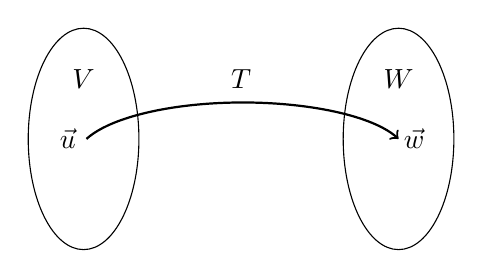
\begin{tikzpicture}
        \draw (2,0) ellipse (20pt and 40pt);
        \draw[] (-2,0) ellipse (20pt and 40pt);
        \draw[<-, thick] (2,0) arc (20:160: 60pt and 20pt);
        \draw (0,1)  node[anchor = north] {$T$};
        \draw (2,1)  node[anchor = north] {$W$}; 
        \draw (-2,1) node[anchor = north] {$V$};
        \draw (-2.2,0) node {$\vec u$};
        \draw (2.2,0) node {$\vec w$};
    \end{tikzpicture}
\end{center}
Recall this diagram, we want to understand $T$ ``correctly". Pick a basis $\li{\vec v}n$ for $V$ and $\li{\vec w}m$ for $W$. We can see that $\dim V = n$ and $\dim W = m$. We can define $T$ as
\[Tv_j = A_{1,j} \vec w_1 + A_{2,j} \vec w_2 + \cdots + A_{m,j} \vec w_m \]
Notice that $A$ has the following form
\[ \begin{array}{cc}
     \vec w_1 \to \\
     \vec w_2 \to \\
     \vdots \\
     \vec w_m \to
\end{array}\bml A_{1,1} & A_{1,2} & \cdots & A_{1,n} \\ 
A_{2,1} & A_{2,2} & \cdots & A_{2,n} \\
\vdots & \vdots & \ddots & \vdots \\ 
A_{m,1} & A_{m,2} & \cdots & A_{m,n} \bmr\]
This is called the matrix representation of $T$.
\begin{example}
    Let $D: V \to W$ be defined as $D := p \to p'$. Let $V:= \spa (1, \cos x, \sin x, \cos 2x, \sin 2x) = W$. We can see that 
    \[\begin{array}{rl}
         1 &\hspace{-0.25cm}\mapsto 0 \\ \cos x &\hspace{-0.25cm}\mapsto -\sin x \\ \sin x &\hspace{-0.25cm}\mapsto \cos x \\ \cos 2x &\hspace{-0.25cm}\mapsto -2 \sin 2x \\ \sin 2x &\hspace{-0.25cm}\mapsto \cos 2x
    \end{array} A = \bml 0 & 0 & 0 & 0 & 0 \\ 
               0 & 0 & -1 & 0 & 0 \\
               0 & 1 & 0 & 0 & 0 \\
               0 & 0 & 0 & 0 & -2 \\
               0 & 0 & 0 & 2 & 0 \bmr\]
\end{example}
\subsection{Matrix Representation} 
Recall that if $T$ is a linear transformation
\begin{center}
    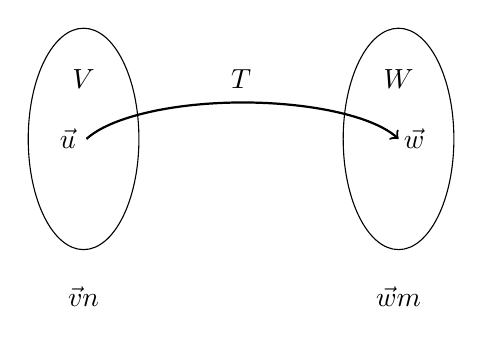
\begin{tikzpicture}
        \draw (2,0) ellipse (20pt and 40pt);
        \draw[] (-2,0) ellipse (20pt and 40pt);
        \draw[<-, thick] (2,0) arc (20:160: 60pt and 20pt);
        \draw (0,1)  node[anchor = north] {$T$};
        \draw (2,1)  node[anchor = north] {$W$}; 
        \draw (-2,1) node[anchor = north] {$V$};
        \draw (-2.2,0) node {$\vec u$};
        \draw (2.2,0) node {$\vec w$};
        \draw (-2, -2) node {$\li{\vec v}n$};
        \draw (2, -2) node {$\li{\vec w}m$};
    \end{tikzpicture}
\end{center}
\[ T\vec v_u = \sum_{k = 1}^{m} A_{i,k} \vec w_k \]
Note that Matrix $A = \left[ A_{i,k} \right]$ has $m$ rows $n$ columns.
\[\left[ \begin{array}{cccc} A_{1,1} & A_{1,2} & \cdots & A_{1,n} \\
        A_{2,1} & A_{2,2} & \cdots & A_{2,n} \\
        \vdots & \vdots & \ddots & \vdots  \\
        A_{m,1} & A_{m,2} & \cdots & A_{m,n} \\
        \end{array} \right]\]
Suppose $v = \lincomb{c}{\vec v}{n}, T\vec v = \lincomb{c}{T\vec v}{n}$.
\[T\vec v =  c_1 \sum_{i=1}^m A_{i,1} \vec w_1  +  c_2 \sum_{i=1}^m A_{i,2} \vec w_2 + \cdots + c_n \sum_{i=1}^m A_{i,n} \vec w_n = \sum_{i = 1}^m \left( \sum_{i = 1}^n A_{i,j} c_j \right) \vec w_j \]
Notice that the operation is the equivalent as the matrix-vector multiplication.
\begin{center}
    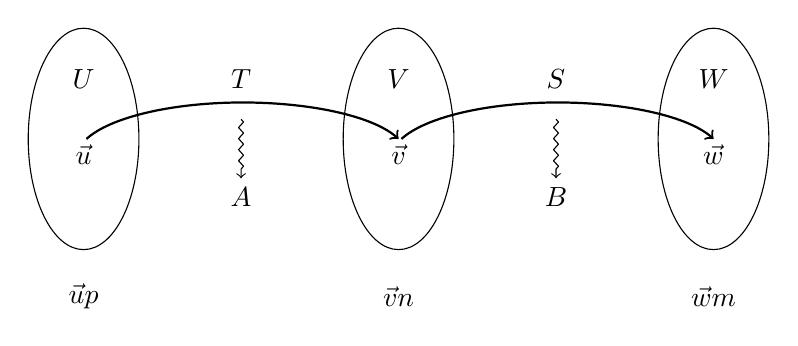
\begin{tikzpicture}
        \draw (2,0) ellipse (20pt and 40pt);
        \draw (-2,0) ellipse (20pt and 40pt);
        \draw (6,0) ellipse (20pt and 40pt);
        \draw[<-, thick] (2,0) arc (20:160: 60pt and 20pt);
        \draw[<-, thick] (6,0) arc (20:160: 60pt and 20pt);
        \draw (0,1)  node[anchor = north] {$T$};
        
        \draw (2,1)  node[anchor = north] {$V$}; 
        \draw (-2,1) node[anchor = north] {$U$};
        \draw (6,1) node[anchor = north] {$W$};
        \draw (4,1) node[anchor = north] {$S$};
        \draw[->, line join=round, decorate, decoration={
    zigzag, segment length=4,
    amplitude=.9,post=lineto,
    post length=2pt }] (0,0.25) -- (0,-0.5);
        \draw[->, line join=round, decorate, decoration={
    zigzag, segment length=4,
    amplitude=.9,post=lineto,
    post length=2pt }] (4,0.25) -- (4,-0.5);
        \draw (0,-0.5) node[anchor = north] {$A$};
        \draw (4,-0.5) node[anchor = north] {$B$};

        \draw (-2,-0.2) node {$\vec u$};
        \draw (2, -0.2) node {$\vec v$};
        \draw (6, -0.2) node {$\vec w$};
        \draw (-2, -2) node {$\li{\vec u}p$};
        \draw (2, -2) node {$\li{\vec v}n$};
        \draw (6, -2) node {$\li{\vec w}m$};
    \end{tikzpicture}
\end{center}
\[ ST\vec u_k = S(T\vec u_k) = S \left( \sum_{j=1}^n A_{j,k}\vec v_j \right) = \sum_{j = 1}^{n} A_{j,k} \left(S\vec v_j\right) = \sum_{j = 1}^n A_{j,k} \sum_{i = 1}^{m} B_{i,j} \vec w_i = \sum_{i = 1}^m \left( \sum_{j = 1}^n B_{i,j}A_{j,k} \right) \vec w_i\]
Use name $\c M(S) := B$, $\c M(T) := A$, $\c M(ST) = BA = \c M(S) \cdot \c M(T)$.
So matrix representation multiply as matrices to produce a composition map or product.
\begin{remark}[Book Keeping]
    $A_{\ast, j}$ denotes the $j$th column of $A$. \\
    $A_{i, \ast}$ denotes the $i$th row of $A$.
\end{remark}
Notice that $\c M$ is a linear map, $\c L (V,W) \xrightarrow{\c M} \b F^{m,n}$. 
\begin{proposition}
    $\c M$ is a linear map.
\end{proposition}

\begin{proposition}
    $\b F^{m,n}$ has a basis.
\end{proposition}
\begin{proof}
    Consider $E_{i,j}$, the matrix consists of all zeros with the exception of $1$ in position $(i,j)$. This can be done for all $i = 1, 2, \ldots, m$, $j  =1,2, \ldots, n$. Also notice that $\dim \b F^{m,n} = m \cdot n$
\end{proof}

\subsection{Invertibility and Isomorphism}
\begin{center}
    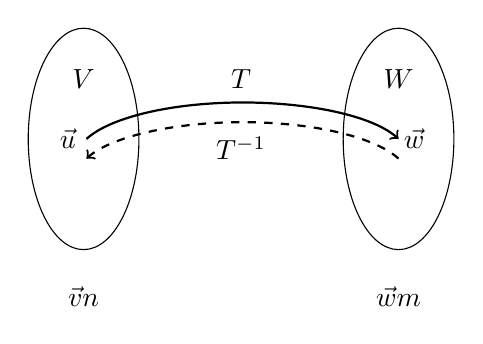
\begin{tikzpicture}
        \draw (2,0) ellipse (20pt and 40pt);
        \draw[] (-2,0) ellipse (20pt and 40pt);
        \draw[<-, thick] (2,0) arc (20:160: 60pt and 20pt);
        \draw[->, thick,style = dashed] (2,-0.25) arc (20:160: 60pt and 20pt);
        \draw (0,1)  node[anchor = north] {$T$};
        \draw (0,0.15)  node[anchor = north] {$T^{-1}$};
        \draw (2,1)  node[anchor = north] {$W$}; 
        \draw (-2,1) node[anchor = north] {$V$};
        \draw (-2.2,0) node {$\vec u$};
        \draw (2.2,0) node {$\vec w$};
        \draw (-2, -2) node {$\li{\vec v}n$};
        \draw (2, -2) node {$\li{\vec w}m$};
    \end{tikzpicture}
\end{center}
\begin{definition}
    $T \in \c L(V,W)$ is invertible provided that there exists a mapping $T^{-1}$ from $W$ to $V$ (not necessarily linear) such that \[ T^{-1} \circ T = \b I_V\]
    \[ T \circ T^{-1} = \b I_W\]
    Where $\b I_{V}, \b I_W$ is the identity map on $V$ and $W$.
\end{definition}
\begin{theorem}
    $T$ is invertible if and only if $T$ is both injective and surjective.
\end{theorem}
\begin{proof}
    Suppose $T$ is invertible, then $T(T^{-1} \vec w) = \vec w \ \forall \vec w \in W$, so $\range T = W$. Also we know that $T^{-1}(T \vec v) = \vec v$. Suppose $T\vec v_1 =T\vec v_2$, apply the left inverse and we have $T^{-1} (T\vec v_1) = T^{-1} (T\vec v_2) \implies \vec v_1 = \vec v_2$. Hence $T$ is injective. Therefore $T$ is bijective. \\
    Now suppose $T$ is bijective. We want to construct $T^{-1}$
    \begin{center}
    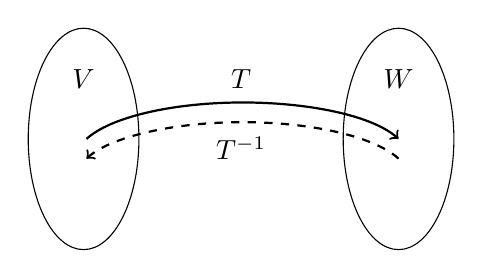
\begin{tikzpicture}
        \draw (2,0) ellipse (20pt and 40pt);
        \draw[] (-2,0) ellipse (20pt and 40pt);
        \draw[<-, thick] (2,0) arc (20:160: 60pt and 20pt);
        \draw[->, thick,style = dashed] (2,-0.25) arc (20:160: 60pt and 20pt);
        \draw (0,1)  node[anchor = north] {$T$};
        \draw (0,0.15)  node[anchor = north] {$T^{-1}$};
        \draw (2,1)  node[anchor = north] {$W$}; 
        \draw (-2,1) node[anchor = north] {$V$};
    \end{tikzpicture}
\end{center}
We need to take $\vec w \in W$, there is a $\vec v \in V$ such that $T\vec v = \vec w$ and such $\vec v$ is unique since $T$ is injective. We declare $T^{-1}\vec w$ to be $\vec v$. So $T^{-1} \circ T = \b I_{V}$. We compute \[ (T \circ T^{-1}) \vec w = T(T^{-1} \vec w) = T\vec v = \vec w \ \forall  \vec w \in W\] So $T \circ T^{-1} = \b I_W$ 
\end{proof}
\begin{definition}
    If $V,W$ are vector spaces, such that there exists a invertible linear map $T \in \c L(V,W)$ then $V, W$ are isomorphic.
\end{definition}
\begin{remark}
    Before we proceed, we want to check that $T^{-1}$ is a linear map when $T \in \c L(V,W)$ and $T^{-1}$ exists.
\end{remark}
\begin{proof}
    Take $\vec w_1,\vec w_2 \in W, \lambda \in \b F$. We compute
    $T^{-1} (\lambda \vec w_1 + \vec w_2)$. We know that $\vec w_1 = T\vec v_1$ and $\vec w_2 = T\vec v_2$. Then we know that $T(\lambda \vec v_1  + \lambda \vec v_2) = \lambda T\vec v_1 + T\vec v_2 = \lambda\vec  w_1 +\vec  w_2$. Subsitute this into $T^{-1}$ and we get
    \[ T^{-1} (\lambda \vec w_1 + \vec w_2) = T^{-1} \circ T (\lambda \vec v_1 + \vec v_2) = \b I (\lambda \vec v_1 + \vec v_2) = \lambda \vec v_1 + \vec v_2 = \lambda T^{-1} \vec w_1 + T^{-1} \vec w_2\] Hence $T^{-1}$ is linear.
\end{proof}
\begin{corollary}
    $\c M$ is actually a bijection between $\c L(V,W)$ and $\b F^{m,n}$, therefore $\c L(V,W)$ is isomorphic to $\b F^{m,n}$.
\end{corollary}
\begin{theorem}
    Suppose $T \in \c L(V,W)$ is linear and invertible, and let $\li {\vec v}m$ be a basis for $V$. Then $\li{T\vec v}n$ is a basis for $W$.
\end{theorem}
\begin{proof}
    Suppose $\lincomb{\alpha}{T\vec v}{n} = 0$. Then $T(\lincomb{\alpha}{\vec v}{n}) = 0$. Since $T$ is injective, this implies $\lincomb{\alpha}{\vec v}{n} = 0$. Therefore $\alpha_1 = \alpha_2 = \cdots = \alpha_n = 0$ since $\li{\vec v}n$ is a basis. Take $\vec w \in W$, then there exists a unique $\vec v \in V$ such that $T\vec v = \vec w$, and $\vec v = \lincomb{\alpha}{\vec v}{n}$ for some $\li \alpha n$, so $T\vec v = \vec w = \lincomb{\alpha}{T\vec v}{n}$, hence span. 
\end{proof}
\begin{corollary}
    $\dim$ is invariant under isomorphism.
\end{corollary}
\subsubsection{Linear Operators}
We are dealing with a specific case where $\c L(V,W)$ is replaced by $\c L(V,V)$.
\begin{center}
    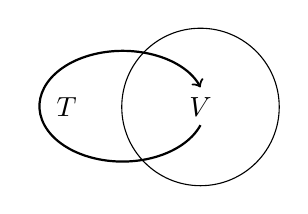
\begin{tikzpicture}
        \draw[<-, thick] (0,0.25) arc (20:340: 30pt and 20pt);
        \draw (0,0) circle(1);
        \draw (0,0) node{$V$};
        \draw (-1.7,0) node{$T$};
    \end{tikzpicture}
\end{center}
Recall that $\dim V = \dim \nul T + \dim \range T$. This gives a better test for invertablity if $W  = V$. 
\begin{theorem}
    Let $T \in \c L(V,V)$. If $V$ is finite dimensional vector space, then the following are equivalent: 
    \begin{enumerate}[label = (\alph*)]
        \item $T$ is injective.
        \item $T$ is surjective.
        \item $T$ is invertible.
    \end{enumerate}
\end{theorem}
\begin{proof} $ $ \\
    (a) $\implies$ (c). Trivial by definition. \\
    (b) $\implies$ (c). Suppose $T$ is injective $\xRightarrow[T \text{ being linear}]{} \nul T = \lb 0 \rb \iff \dim \nul T = 0$. Therefore 
    \[ \dim V = \dim \nul T = \dim \range T = 0\] So $\dim V = \dim \range T$, hence $\range T = V$, so $T$ is surjective. \\
    (c) $\implies$ (a).  \[\dim V = \dim \nul T + \dim \range T = \dim \nul T + \dim V \implies \dim \nul T  = 0 \implies \nul T = \lb \vec 0 \rb\] So $T$ is injective. $T$ is already known to be surjective, so $T$ is bijective, or $T$ is invertable.
\end{proof}
\begin{example}
    The theorem does not hold for infinite dimension vector spaces, for example: \\ 
    The differentiation map $T : f(x) \mapsto f'(x)$ is surjective but not invertible over $\c P(\b R)$.  From calculus we know that for every $f(x) \in \c P(\b R)$, there exists $g(x) \in \c P(\b R)$ such that $g'(x) = f(x)$, however, we can see that $\nul T \neq \lb 0 \rb$ as $1 \in
    \nul T$. Hence $T$ is not injective. \\
    The integration map $\displaystyle T: f(x) \mapsto \int_0^x f(t) dt$ is injective but not invertible over $\c P(\b R)$. We can see that $\nul T = \lb 0 \rb$, hence $T$ is injective, however, $1 \not\in \range T$.
\end{example}
\subsection{Duality}
\begin{definition}
    Given a vector space $V$, we define its dual space as $V' = \c L(V,\b F)$. 
\end{definition}
\begin{remark}
    Objects in $\c L(V,\b F)$ are also called linear functional.
\end{remark}
\begin{example}
    Linear Functional on $\b R^3$: $(x_1, x_2, x_3) \mapsto \alpha_1 x_1 + \alpha_2 x_2 + \alpha_3 x_3 \ \forall \alpha_1, \alpha_2, \alpha_3 \in \b R$.
\end{example}
\begin{definition}
    Suppose $\li{\vec v}n$ is a basis of $V$. The list of linear functionals $\li \varphi n \in  V'$ such that \[\varphi_i(\vec v_j) = \left\{ \begin{array}{cc}
         1 \text{ if } i = j \\
         0 \text{ if } i \neq j
    \end{array} \right.\] We claim that $\li\varphi n$ is the dual basis of $V'$.
\end{definition}
\begin{lemma}
    A dual basis is a basis of $V'$.
\end{lemma}
\begin{proof}
    Suppose there exists $\li \alpha n$ such that 
    \[ \lincomb{\alpha}{\varphi}{n} = 0\]
    We compute for $v_1$
    \[ (\lincomb{\alpha}{\varphi}{n})(n) = \alpha_1 \cdot 1 + 0 \implies \alpha_1 = 0\]
    Similarly, if we plug in an arbitrary $v_j$
    \[ (\lincomb{\alpha}{\varphi}{n})\vec v_j) \implies v_j = 0\]
    This shows that $\li \varphi n$ is linear independent, and the count is $n$. So $\li \varphi n$ form a basis for $V'$.
\end{proof}
\subsubsection{Dual Maps}
\begin{center}
    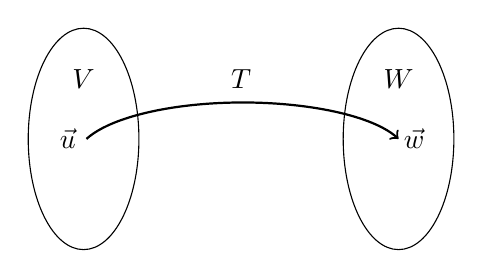
\begin{tikzpicture}
        \draw (2,0) ellipse (20pt and 40pt);
        \draw[] (-2,0) ellipse (20pt and 40pt);
        \draw[<-, thick] (2,0) arc (20:160: 60pt and 20pt);
        \draw (0,1)  node[anchor = north] {$T$};
        \draw (2,1)  node[anchor = north] {$W$}; 
        \draw (-2,1) node[anchor = north] {$V$};
        \draw (-2.2,0) node {$\vec u$};
        \draw (2.2,0) node {$\vec w$};
    \end{tikzpicture}
\end{center}
\begin{center}
    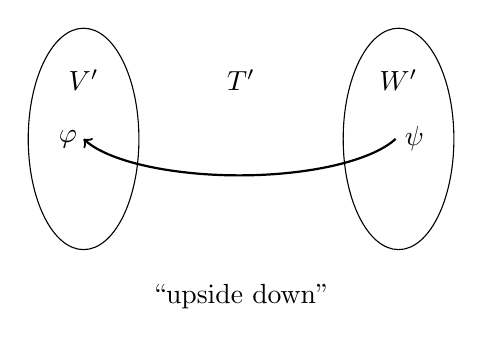
\begin{tikzpicture}
        \draw (2,0) ellipse (20pt and 40pt);
        \draw[] (-2,0) ellipse (20pt and 40pt);
        \draw[<-, thick] (-2,0) arc (200:340: 60pt and 20pt);
        \draw (0,1)  node[anchor = north] {$T'$};
        \draw (2,1)  node[anchor = north] {$W'$}; 
        \draw (-2,1) node[anchor = north] {$V'$};
        \draw (-2.2,0) node {$\varphi$};
        \draw (2.2,0) node {$\psi$};
        \draw (0, -2) node {``upside down"};
    \end{tikzpicture}
\end{center}
\begin{definition}
    Given $T \in \c L(V,W)$, we define $T' : \varphi \mapsto \varphi \circ T$. $ \phi \in W'$ i.e. $\varphi \in \c L(W, \b F)$. Notice that $\varphi \circ T \in \c L(V, \b F)$.
\end{definition}
\begin{example}
    Define $V, W, \varphi, T$ as $\varphi : f \mapsto \int_0^1 f(t) dt, V = \c P_3(\b R), W = \c P_2(\b R), T : f \mapsto f'$. What is $\varphi \circ T$? 
    \[ (\varphi \circ T)(f) = \varphi(T(f)) = \varphi (f') = \int_0^1 f'(t)dt = f(1) - f(0)\]
\end{example}
\begin{remark}[Algebraic Property of dual maps] $ $
    \vspace{-0.5cm}
    \begin{enumerate}
        \item $(S + T)'  = S' + T'$
        \begin{proof}
            For any $S,T \in \c L(V,W), S', T' \in \c L(W',V')$ , we compute 
            \[(S + T)'(\varphi) = \varphi \circ (S + T) = \varphi \circ S + \varphi \circ T = S'(\varphi) + T'(\varphi)\]
        \end{proof}
        \item $(\lambda S)' = \lambda S'$
        \begin{proof}
            \[ (\lambda S)'(\varphi) = \varphi \circ (\lambda S) = \lambda (\varphi \circ S) = \lambda \cdot S'(\varphi)\]
        \end{proof}
        \item $(ST)'  = T' S'$
        \begin{proof}
            Sanity check: $S \in \c L(V,W), T \in \c L(U,V)$
            \[ (ST)' : \varphi \mapsto \varphi 
            \circ (ST) = (\varphi \circ S) \circ T = T'(\varphi \circ S) = T'(S'(\varphi)) = T' \circ S'\]
        \end{proof}
    \end{enumerate}
\end{remark}
\begin{definition}[Annihilators]
    Let a set $S$ to be a subset of a vector space $V$. We can define $S^0$ as 
    \[ S^0 := \lb \varphi \in V' : \varphi (v) = 0 \ \forall \vec v \in S \rb\]
\end{definition}
\begin{example}
    Consider $\b R^3$, let $S := \lb (1,0,0), (1,1,0) \rb$. We know that any $\varphi \in \b R^3$ will have the form of $(x_1,x_2,x_3) \mapsto a_1x_1 + a_2x_2 + a_3x_3$ for some constant $a_1,a_2,a_3$. Plug in $(1,0,0)$ and $(1,1,0)$ and we get 
    \[ a_1 \cdot 1 + a_2 \cdot 0 + a_3 \cdot 0 = 0 \implies a_1 = 0\]
    \[ a_1 \cdot 1 + a_2 \cdot 1 + a_3 \cdot 0 = 0 \implies a_2 = 0\]
    We can see that $S^{0} = \lb \varphi(x_1, x_2, x_3) = a_3 x_3 \text{ for some } a_3 \in \b R \rb$ and forms a subspace for $\b R^{3}$'.
\end{example}
\begin{lemma}
    Regardless of the nature of $S$, $S^0$ is always a subspace.
\end{lemma}
\newpage
\begin{proof}
    \begin{enumerate}
        \item The zero functional is clearly in $S^0$.
        \item Suppose $\varphi \in S^0$, take $\lambda \in \b F$, then $(\lambda \varphi)(\vec v) = \lambda \cdot \varphi(\vec v) = 0$ for all $\vec v \in S$. So $\lambda \varphi \in S$.
        \item Suppose $\varphi, \psi \in S^0$, then $(\varphi + \psi)(\vec v) = \varphi(\vec v) + \psi(\vec v) = 0$ for all $\vec v \in S$. Therefore $\varphi + \psi \in S^0$.
    \end{enumerate}
\end{proof}
\begin{theorem}
    Suppose $S = U$, where $U$ is a subspace of $V$, then 
    \[ \dim U + \dim U^0 = \dim V\]
\end{theorem}
\begin{proof}
    Consider the inclusion map: \[i : U \to V : \vec u \to \vec u \ \forall \vec u \in U\] 
    Take  a look at the dual of $U$: $i' \in \c L(V', U')$. Apply Rank-Nullity to the dual map and we can see that $\dim V' = \dim \nul i' + \dim \range i'$. We also know that \[\nul i' = \lb \varphi \in V' : \varphi \circ i = 0 \rb\] Notice that $\varphi \circ i = 0$ as a functional implies \[(\varphi \circ i) (\vec u) = 0 \implies \varphi(i(\vec u)) = 0 \implies \varphi(\vec u) = 0 \ \forall \vec u \in U \]
    Therefore we can see that $\range i' = \lb \varphi \circ i : \varphi \in V' \rb = U'$ since any linear functional on $U$ extends to $V$. I have a clever proof for this but it does not fit in the margin of the page and is left as an exercise for the reader. 
\end{proof}
\begin{theorem}
    Let $V,W$ be finite dimensional vector space and let $T \in \c L(V,W)$. Then 
    \begin{enumerate}[label = (\alph*)]
        \item $\nul T' = (\range T)^0$
        \item $\dim \nul T' = \dim \nul T + \dim W - \dim V$
    \end{enumerate}
\end{theorem}
\begin{proof} $ $
    \begin{enumerate}[label = (\alph*)]
        \item $\varphi \in \nul T' \iff \varphi \circ T = 0 \iff (\varphi \circ T)(\vec v) = 0 \ \forall \vec v \in V \iff \varphi(T\vec v) = 0 \ \forall \vec v \in V \\ \iff \varphi \in (\range T)^0$
        \item $\dim \nul T' = \dim (\range T)^0 = \dim W - \dim \range T = \dim W - (\dim V - \dim \nul T) = \dim W - \dim V + \dim \nul T$
    \end{enumerate}
\end{proof}
\begin{corollary}
    $T'$ is injective if and only if $T$ is surjective.
\end{corollary}
\begin{theorem}
    Suppose $V$ and $W$ are finite dimensional and $T \in \c L(V,W)$, then 
    \begin{enumerate}[label = (\alph*)]
        \item $\dim \range T' = \dim \range T$
        \item $\range T' = (\nul T)^0$
    \end{enumerate}
\end{theorem}
\begin{proof} $ $
    \begin{enumerate}[label = (\alph*)]
        \item $\dim \range T' = \dim W' - \dim \nul T' = \dim W - (\dim W - \dim V + \dim \nul T) = \dim V - \dim \nul T = \dim \range T$
        \item $\psi \in \range T' \iff \exists \varphi : \varphi \circ T = \psi \iff \varphi \circ T(\vec v) = \psi(\vec v) \ \forall \vec v \in V \iff \varphi(T\vec v) = \psi(\vec v) \forall \vec v \in V$. \\ So $T\vec v = 0 \implies \psi(\vec v) = 0$. This shows $\range T' \subseteq (\nul T)^0$. But $\dim \range T' = \dim \range T = \dim V - \dim \nul T = \dim (\nul T)^0$. Hence $\range T = \nul T$.
    \end{enumerate}
\end{proof}
\subsubsection{Matrix Representation of the dual map}
Recall that
\begin{center}
    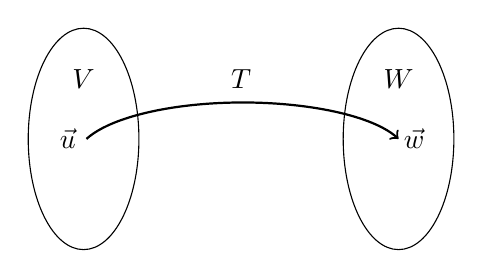
\begin{tikzpicture}
        \draw (2,0) ellipse (20pt and 40pt);
        \draw[] (-2,0) ellipse (20pt and 40pt);
        \draw[<-, thick] (2,0) arc (20:160: 60pt and 20pt);
        \draw (0,1)  node[anchor = north] {$T$};
        \draw (2,1)  node[anchor = north] {$W$}; 
        \draw (-2,1) node[anchor = north] {$V$};
        \draw (-2.2,0) node {$\vec u$};
        \draw (2.2,0) node {$\vec w$};
    \end{tikzpicture}
\end{center}
\begin{center}
    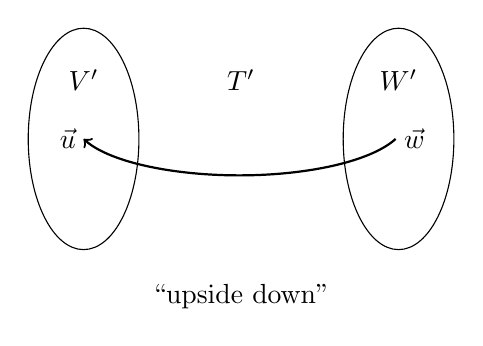
\begin{tikzpicture}
        \draw (2,0) ellipse (20pt and 40pt);
        \draw[] (-2,0) ellipse (20pt and 40pt);
        \draw[<-, thick] (-2,0) arc (200:340: 60pt and 20pt);
        \draw (0,1)  node[anchor = north] {$T'$};
        \draw (2,1)  node[anchor = north] {$W'$}; 
        \draw (-2,1) node[anchor = north] {$V'$};
        \draw (-2.2,0) node {$\vec u$};
        \draw (2.2,0) node {$\vec w$};
        \draw (0, -2) node {``upside down"};
    \end{tikzpicture}
\end{center}
We also recall that $T' : \varphi \mapsto \varphi \circ T$.
\newpage
\begin{question}
    How do we get $\c M(T')$ given $\c M(T)$?
\end{question}
\begin{answer}
For $\c M(T)$, we need $2$ bases $\li {\vec v}n$ for $V$ and $\li {\vec w}m$ for $W$. \\
    Take $\li \varphi n$, a dual basis to $\li {\vec v}n$, it is a basis for $V'$. \\
    Tale $\li \psi m$, a dual basis to $\li {\vec w}m$, it is a basis for $W'$. \\
    Given $\c M(T)$, we want to construct / understand $\c M(T')$with regard to the basis $\li \psi m$ of $W'$ and $\li \varphi n$ of $V'$. \\
    We know $\c M(T)$ has $m$ rows $n$ columns, and $\c M(T')$ has $n$ rows and $m$ columns. \\Suppose $\c M(T) = A, \c M(T') = C$, we then know 
    \[ T\vec v_j = \sum_{i = 1}^m A_{i,j} \vec w_i \ \forall j = 1,2, \ldots, n, T'\psi_l = \sum_{l = 1}^n C_{l,k} \varphi_{l} \ \forall l =  1,2,\ldots, m\]
    \[ T' \psi_k = \psi_k \circ T \implies (\psi_k \circ T )(\vec v_j) = \psi_k(T\vec v_j) = \psi_k \left( \sum_{i=1}^m A_{i,j} \vec w_j \right) = \sum_{i = 1}^m A_{i,j} \psi_k(\vec w_i) = \sum_{i = 1}^m A_{i,j} \delta_{ki} = A_{k,j}\]
    \[(T'\psi_k)(\vec v_j) = \left( \sum_{l = 1}^{n} C_{l,k} \varphi_l \right) (\vec v_j) = \sum_{l = 1}^{n} C_{l,k} \varphi(\vec v_j) = \sum_{l = 1}^{n} C_{l,k} \delta_{l,j} = C_{j,k} \]
    Notice that $A_{k,j} = C_{j,k} \ \forall j,k$.
\end{answer}
\begin{conjecture}
    So we obtained that 
    \[ M(T') = M(T)^{T}\]
    provided that the basis of $V'$ and $W'$ are chosen to be the dual to the bases of $V$ and $W$, respectively.
\end{conjecture}
\begin{example}
    Let $T: p \mapsto p'$ for $V = \c P_3(\b R)$ with basis $1,x,x^2, X^3$, and $W = \c P_2(\b R)$ with $1,x,x^2$. \\
    We can see that the dual basis for $1,x,x^2, x^3$ is \[\varphi_0 : p \mapsto p(0), \varphi_1 : p \mapsto p'(0), \varphi_2: p \mapsto \frac{p''(0)}{2}, \varphi_3 : p \mapsto \frac{p'''(0)}{3!}\]
    Dual basis for $1,x,x^2$ is 
    \[\psi_0 : p \mapsto p(0), \psi_1 : p \mapsto p'(0), \psi_2: p \mapsto \frac{p''(0)}{2}, 
    \]
    Notice that \[\c M(T) = \bml 0 & 1 & 0 & 0 \\ 0 & 0 & 2 & 0 \\ 0 & 0 & 0 & 3\ \bmr \text{ and } \c M(T') = \bml 0 & 0 & 0 \\ 1 & 0 & 0 \\ 0 & 2 & 0 \\ 0 & 0 & 3 \bmr\]
\end{example}